\subsection{Phân bổ nguồn lực (Resource Allocation)}
\label{sec:resource-allocation}

Dựa trên cấu trúc phân rã công việc (WBS tại Mục 2.7) và kế hoạch quản lý rủi ro (Mục 2.9), tổng khối lượng công việc của dự án là 331,6 giờ công, triển khai từ ngày 26/10/2026 đến ngày 06/12/2026. Nguồn lực được phân bổ dựa trên Capacity thực tế của từng nhân sự, thời gian cho các hoạt động quản lý định kỳ và khả năng sẵn sàng của hạ tầng dùng chung. Lịch trình công việc được sắp xếp theo trình tự phụ thuộc hợp lý, hướng tới mốc bàn giao sản phẩm ngày 03/12/2026 và dành 3 ngày cuối (04--06/12/2026) làm dự phòng tiến độ (Schedule Buffer).

\subsubsection{Khả năng tham gia (Capacity)}

Capacity ($C_{i,w}$) phản ánh quỹ thời gian tối đa mà thành viên $i$ cam kết dành cho dự án trong tuần $w$ sau khi đã trừ lịch học và việc cá nhân. Quỹ thời gian khả dụng cho các tác vụ kỹ thuật chuyên môn ($C^{\mathrm{khac}}_{i,w}$) được tính bằng cách trừ đi thời gian cố định cho công tác theo dõi tiến độ (G05) và rà soát rủi ro (G06):
\[C^{\mathrm{khac}}_{i,w}=C_{i,w}-h_{G05,i,w}-h_{G06,i,w}.\]

\begingroup\small
\setlength{\tabcolsep}{4pt}\renewcommand{\arraystretch}{1.15}
\begin{longtable}{@{}l*{7}{r}@{}}
\caption{Giới hạn Capacity theo tuần của từng nhân sự (Đơn vị: Giờ công)}\label{tab:capacity}\\
\toprule
\textbf{Nhân sự} & \textbf{T1} & \textbf{T2} & \textbf{T3} & \textbf{T4} & \textbf{T5} & \textbf{T6} & \textbf{Tổng} \\
\midrule\endfirsthead
\toprule
\textbf{Nhân sự} & \textbf{T1} & \textbf{T2} & \textbf{T3} & \textbf{T4} & \textbf{T5} & \textbf{T6} & \textbf{Tổng} \\
\midrule\endhead
\midrule\multicolumn{8}{r}{\textit{Còn tiếp}}\\\endfoot
\bottomrule\endlastfoot
PM & 15,0 & 14,0 & 14,0 & 13,0 & 12,0 & 12,0 & 80,0 \\
BA & 14,0 & 13,0 & 13,0 & 12,0 & 12,0 & 12,0 & 76,0 \\
BE & 13,0 & 15,0 & 14,0 & 13,0 & 12,0 & 12,0 & 79,0 \\
FE & 12,0 & 15,0 & 14,0 & 13,0 & 12,0 & 12,0 & 78,0 \\
QA & 13,0 & 12,0 & 13,0 & 16,0 & 14,0 & 14,0 & 82,0 \\
\textbf{Tổng} & \textbf{67,0} & \textbf{69,0} & \textbf{68,0} & \textbf{67,0} & \textbf{62,0} & \textbf{62,0} & \textbf{395,0} \\
\end{longtable}\endgroup

Dự án bố trí các khung giờ làm việc linh hoạt P1/P2 từ thứ Hai đến thứ Bảy (tối đa 2 giờ/người/phiên) dựa trên thời khóa biểu cá nhân. Ngày Chủ nhật là ngày nghỉ kế hoạch.

Ví dụ ở Tuần 2, QA có Capacity là 12,0 giờ công. Sau khi trừ 1,1 giờ làm nhiệm vụ quản lý (G05, G06), QA còn 10,9 giờ khả dụng cho các việc chuyên môn. Các công việc dự phòng rủi ro (RA01--RA06) cũng được tính trực tiếp vào tổng ngân sách giờ công này.

\subsubsection{Phân bổ công việc (Effort Allocation)}

Tổng công sức kế hoạch 331,6 giờ công được chia thành ba nhóm:
\[E = 250{,}0 \text{ (Kỹ thuật/Bàn giao)} + 70{,}5 \text{ (Quản lý/Lập kế hoạch)} + 11{,}1 \text{ (Tác vụ RA)} = 331{,}6\text{ giờ công}.\]

Bảng 43 tổng hợp phân công chi tiết theo từng hoạt động. Trong đó, gói BL1 thay thế cho A04.2, A04.3 và gói BL2 thay thế cho A13, A14.2 để tối ưu quản lý.

\begingroup\small
\setlength{\tabcolsep}{4pt}\renewcommand{\arraystretch}{1.15}
\begin{longtable}{@{}lp{.30\linewidth}*{6}{r}@{}}
\caption{Phân công khối lượng công việc theo hoạt động (Đơn vị: Giờ công)}\label{tab:allocation}\\
\toprule
\textbf{Mã} & \textbf{Hoạt động} & \textbf{PM} & \textbf{BA} & \textbf{BE} & \textbf{FE} & \textbf{QA} & \textbf{Tổng} \\
\midrule\endfirsthead
\toprule
\textbf{Mã} & \textbf{Hoạt động} & \textbf{PM} & \textbf{BA} & \textbf{BE} & \textbf{FE} & \textbf{QA} & \textbf{Tổng} \\
\midrule\endhead
\midrule\multicolumn{8}{r}{\textit{Còn tiếp}}\\\endfoot
\bottomrule\endlastfoot
A01 & Thiết kế CSDL, giao diện, API & 0,0 & 7,0 & 6,0 & 1,0 & 2,0 & 16,0 \\
A02.1 & Test case Increment 1 & 0,0 & 2,0 & 0,0 & 0,0 & 3,0 & 5,0 \\
A02.2 & Test case Increment 2 & 0,0 & 1,0 & 0,0 & 0,0 & 2,5 & 3,5 \\
A02.3 & Test case Increment 3 & 0,0 & 1,0 & 0,0 & 0,0 & 2,5 & 3,5 \\
A03 & Thiết lập môi trường triển khai & 2,0 & 0,0 & 3,0 & 1,0 & 2,0 & 8,0 \\
A04.1 & Dữ liệu thử Increment 1 & 1,0 & 1,0 & 0,0 & 0,0 & 1,5 & 3,5 \\
A05.1 & Lập trình Tài khoản, phân quyền & 0,0 & 8,0 & 10,0 & 0,0 & 0,0 & 18,0 \\
A05.2 & Lập trình Quản lý sự kiện & 6,0 & 0,0 & 0,0 & 10,0 & 2,0 & 18,0 \\
A06 & Kiểm thử, sửa lỗi Increment 1 & 0,0 & 1,0 & 2,0 & 2,0 & 5,0 & 10,0 \\
A07.1 & Lập trình Đăng ký, hủy, sức chứa & 6,0 & 1,0 & 5,0 & 9,0 & 1,0 & 22,0 \\
A07.2 & Lập trình Danh sách chờ FIFO & 0,0 & 1,0 & 5,0 & 7,0 & 1,0 & 14,0 \\
A07.3 & Lập trình Email thông báo & 4,0 & 1,0 & 0,0 & 0,0 & 1,0 & 6,0 \\
A08 & Kiểm thử, sửa lỗi Increment 2 & 0,0 & 1,0 & 3,0 & 3,0 & 6,0 & 13,0 \\
A09.1 & Lập trình Điểm danh QR & 0,0 & 1,0 & 6,0 & 4,0 & 1,0 & 12,0 \\
A09.2 & Lập trình Điểm danh thủ công & 4,0 & 1,0 & 0,0 & 4,0 & 1,0 & 10,0 \\
A10.1 & Lập trình Báo cáo cơ bản & 0,0 & 6,0 & 4,0 & 2,0 & 1,0 & 13,0 \\
A10.2 & Lập trình Xuất CSV/Excel & 4,0 & 0,0 & 0,0 & 0,0 & 1,0 & 5,0 \\
A11 & Tích hợp, triển khai nghiệm thu & 0,0 & 0,0 & 3,0 & 2,0 & 2,0 & 7,0 \\
A12.1 & Integration Test & 1,0 & 0,0 & 4,0 & 3,0 & 6,0 & 14,0 \\
A12.2 & Đo chỉ tiêu, chốt Quality Evidence & 0,0 & 4,0 & 0,0 & 0,0 & 4,0 & 8,0 \\
A14.1 & Soạn thảo User Guide & 0,0 & 1,0 & 1,0 & 1,0 & 0,0 & 3,0 \\
A15.1 & Tổng hợp số liệu đánh giá & 1,0 & 0,5 & 0,0 & 0,0 & 0,5 & 2,0 \\
A15.2 & Chốt Retrospective \& Lessons Learned & 2,0 & 1,5 & 0,5 & 0,5 & 1,5 & 6,0 \\
A16 & Kế hoạch đóng dự án và bàn giao & 2,0 & 1,0 & 0,5 & 0,5 & 1,0 & 5,0 \\
A17 & Demo và bàn giao sản phẩm & 1,0 & 1,0 & 1,0 & 1,0 & 1,0 & 5,0 \\
A18.1 & Tổng hợp bản thảo báo cáo quản lý & 1,0 & 1,0 & 0,0 & 0,0 & 0,5 & 2,5 \\
A18.2 & Chốt báo cáo quản lý dự án & 2,0 & 1,0 & 0,5 & 0,5 & 0,5 & 4,5 \\
A19.1 & Ghi nhận đóng góp, chuẩn bị demo & 0,5 & 0,5 & 0,5 & 0,5 & 0,5 & 2,5 \\
A19.2 & Hoàn thiện Reflection và diễn tập & 0,5 & 0,5 & 0,5 & 0,5 & 0,5 & 2,5 \\
BL1 & Dữ liệu thử Increment 2, 3 & 1,0 & 1,0 & 0,0 & 0,0 & 1,5 & 3,5 \\
BL2 & Chốt phiên bản, xác minh User Guide & 0,0 & 0,0 & 1,0 & 0,5 & 2,5 & 4,0 \\
G02 & Rà soát sản phẩm và phụ thuộc & 3,0 & 3,0 & 1,0 & 1,0 & 2,0 & 10,0 \\
G03 & Ước lượng, lập kế hoạch lịch trình & 5,0 & 2,0 & 1,0 & 1,0 & 2,0 & 11,0 \\
G04 & Phê duyệt Project Baseline V1.0 & 2,0 & 0,5 & 0,5 & 0,5 & 0,5 & 4,0 \\
G05 & Theo dõi và kiểm soát tiến độ & 10,0 & 5,0 & 5,0 & 5,0 & 5,0 & 30,0 \\
G06 & Rà soát và kiểm soát rủi ro & 3,0 & 3,0 & 0,5 & 0,5 & 0,5 & 7,5 \\
G07 & Phân tích và quản lý thay đổi & 3,0 & 2,0 & 1,0 & 1,0 & 1,0 & 8,0 \\
RA01 & Thử nghiệm tải đồng thời và FIFO & 0,0 & 0,0 & 2,0 & 0,0 & 0,5 & 2,5 \\
RA02 & Thử nghiệm triển khai AWS Lightsail & 0,0 & 0,0 & 1,0 & 1,5 & 0,0 & 2,5 \\
RA03 & Thử nghiệm tích hợp dịch vụ Email & 1,0 & 0,0 & 0,0 & 0,0 & 0,0 & 1,0 \\
RA04 & Thử nghiệm sinh và quét mã QR & 0,0 & 0,0 & 0,0 & 1,5 & 0,5 & 2,0 \\
RA05 & Thử nghiệm hiệu năng xuất báo cáo & 0,0 & 0,0 & 0,4 & 0,0 & 1,5 & 1,9 \\
RA06 & Làm rõ yêu cầu kỹ thuật tích hợp & 0,4 & 0,8 & 0,0 & 0,0 & 0,0 & 1,2 \\
\textbf{Tổng} &  & \textbf{66,4} & \textbf{62,3} & \textbf{68,9} & \textbf{65,0} & \textbf{69,0} & \textbf{331,6} \\
\end{longtable}\endgroup

Về phân công chuyên môn: BE chịu trách nhiệm chính mảng Backend và code review (có PM hỗ trợ); FE chịu trách nhiệm chính mảng Frontend và UI (có BA hỗ trợ); QA phụ trách kiểm thử độc lập. Công sức hỗ trợ của PM và BA được tính trực tiếp vào quỹ giờ cá nhân. Khối lượng quản lý định kỳ (G05, G06) duy trì 37,5 giờ công trong 5 tuần. Tác vụ G08 (4,0 giờ công) là khoản dự phòng quản lý khi có thay đổi phát sinh và không nằm trong Baseline 331,6 giờ công.

\subsubsection{Cấu trúc Activity Splitting}

Để giảm thời gian chờ giữa các khâu, nhóm áp dụng kỹ thuật Activity Splitting cho các tác vụ phát triển và kiểm thử.

\begingroup\small
\setlength{\tabcolsep}{4pt}\renewcommand{\arraystretch}{1.15}
\begin{longtable}{@{}lp{.52\linewidth}r@{}}
\caption{Cấu trúc Activity Splitting phục vụ lập lịch}\label{tab:split}\\
\toprule
\textbf{Mã gốc} & \textbf{Mã thực hiện (Splitting)} & \textbf{Công sức (h)} \\
\midrule\endfirsthead
\toprule
\textbf{Mã gốc} & \textbf{Mã thực hiện (Splitting)} & \textbf{Công sức (h)} \\
\midrule\endhead
\midrule\multicolumn{3}{r}{\textit{Còn tiếp}}\\\endfoot
\bottomrule\endlastfoot
A05 & A05.1 (Tài khoản, phân quyền); A05.2 (Quản lý sự kiện) & 18,0; 18,0 \\
A07 & A07.1 (Đăng ký); A07.2 (Hàng chờ FIFO); A07.3 (Email) & 22,0; 14,0; 6,0 \\
A09 & A09.1 (Điểm danh QR); A09.2 (Điểm danh thủ công) & 12,0; 10,0 \\
A10 & A10.1 (Báo cáo cơ bản); A10.2 (Xuất tệp CSV/Excel) & 13,0; 5,0 \\
A12 & A12.1 (Integration Test); A12.2 (Quality Evidence) & 14,0; 8,0 \\
A04.2; A04.3 & Gói gộp BL1 (Dữ liệu thử Increment 2, 3) & 3,5 \\
A13; A14.2 & Gói gộp BL2 (Chốt phiên bản \& User Guide) & 4,0 \\
\end{longtable}\endgroup

Trình tự thực hiện giữa các tác vụ chính được thiết lập như sau:
\begin{itemize}
    \item \textbf{Increment 1:} A05.1 (Tài khoản) và A05.2 (Sự kiện) triển khai song song sau khi hoàn thành A03. Tác vụ rủi ro RA06 phải xong trước mốc CP1.
    \item \textbf{Increment 2:} Thực hiện nối tiếp chuỗi A07.1 $\to$ A07.2 $\to$ A07.3. Trong đó, A07.2 chờ kết quả thử nghiệm RA01 và A07.3 chờ RA03.
    \item \textbf{Increment 3 \& Tích hợp:} Hoạt động A11 bắt đầu sau khi hoàn thành A09.1, A09.2, A10.2 và kết quả triển khai RA02.
    \item \textbf{Bàn giao (BL2):} Việc chốt mã nguồn được thực hiện trước khi rà soát và xác minh User Guide.
\end{itemize}

\subsubsection{Ràng buộc môi trường và hạ tầng}

\begingroup\small
\setlength{\tabcolsep}{4pt}\renewcommand{\arraystretch}{1.15}
\begin{longtable}{@{}p{.22\linewidth}p{.70\linewidth}@{}}
\caption{Điều kiện sử dụng nguồn lực và hạ tầng kỹ thuật}\label{tab:shared}\\
\toprule
\textbf{Nguồn lực} & \textbf{Ràng buộc vận hành và điều kiện sử dụng} \\
\midrule\endfirsthead
\toprule
\textbf{Nguồn lực} & \textbf{Ràng buộc vận hành và điều kiện sử dụng} \\
\midrule\endhead
\midrule\multicolumn{2}{r}{\textit{Còn tiếp}}\\\endfoot
\bottomrule\endlastfoot
Thiết bị cá nhân & Mỗi thành viên tự chuẩn bị phần cứng đáp ứng yêu cầu công việc. \\
AWS Lightsail & Khởi tạo tại A03; thử nghiệm RA02 sau A05.1; giữ ổn định môi trường cho A11 và A12. \\
Môi trường CSDL & Tách biệt bộ dữ liệu thử nghiệm (BL1); giữ nguyên trạng thái phục vụ thu thập Quality Evidence tại A12.2. \\
Thiết bị QR & Thử nghiệm RA04 trước A09.1; phân bổ lịch sử dụng thiết bị đồng bộ giữa FE và QA. \\
Dịch vụ Email & Xác nhận hạn mức dịch vụ RA03 trước A07.3; dùng môi trường Mock cho kiểm thử lặp. \\
Môi trường đo tải & Thực hiện RA05 trên bộ dữ liệu 500 bản ghi nhằm hỗ trợ cho phép đo nghiệm thu A12.2. \\
Khách hàng & Thống nhất lịch làm việc tại các Milestone CP0, CP1, CP4 và CP6. \\
\end{longtable}\endgroup

\subsubsection{San bằng nguồn lực (Resource Leveling)}

Để xử lý tình trạng quá tải nhân sự (Over-allocation), phương pháp Resource Leveling được áp dụng dựa trên điều kiện: tổng giờ phân bổ không vượt quá Capacity ($H_{i,w} \le C_{i,w}$) và lượng quá tải bằng 0 ($O_{i,w} = 0$):
\[H_{i,w}=\sum_a h_{a,i,w}\le C_{i,w},\qquad O_{i,w}=\max(0, H_{i,w}-C_{i,w}).\]

Lịch Early Start ban đầu khiến nhóm bị quá tải 56,2 giờ công (tập trung ở Tuần 1 và Tuần 4). Sau khi dịch chuyển các tác vụ có thời gian dự trữ sang Tuần 2 và Tuần 3, tải làm việc đã được cân bằng hoàn toàn trên cả 6 tuần.

\begingroup\small
\setlength{\tabcolsep}{4pt}\renewcommand{\arraystretch}{1.15}
\begin{longtable}{@{}ll*{7}{r}@{}}
\caption{Phân kỳ công sức giữa phương án Early Start và Resource Leveled (Đơn vị: Giờ công)}\label{tab:weekly}\\
\toprule
\textbf{Nhân sự} & \textbf{Phương án} & \textbf{T1} & \textbf{T2} & \textbf{T3} & \textbf{T4} & \textbf{T5} & \textbf{T6} & \textbf{Tổng} \\
\midrule\endfirsthead
\toprule
\textbf{Nhân sự} & \textbf{Phương án} & \textbf{T1} & \textbf{T2} & \textbf{T3} & \textbf{T4} & \textbf{T5} & \textbf{T6} & \textbf{Tổng} \\
\midrule\endhead
\midrule\multicolumn{9}{r}{\textit{Còn tiếp}}\\\endfoot
\bottomrule\endlastfoot
PM & Early Start & 21,3 & 9,3 & 11,0 & 13,9 & 9,9 & 1,0 & 66,4 \\
PM & Resource Leveled & 15,0 & 11,5 & 12,6 & 12,1 & 7,7 & 7,5 & 66,4 \\
BA & Early Start & 26,4 & 7,7 & 4,9 & 12,6 & 9,7 & 1,0 & 62,3 \\
BA & Resource Leveled & 14,0 & 12,9 & 11,1 & 11,0 & 7,8 & 5,5 & 62,3 \\
BE & Early Start & 20,5 & 7,6 & 13,1 & 19,8 & 6,9 & 1,0 & 68,9 \\
BE & Resource Leveled & 12,5 & 14,4 & 13,8 & 12,0 & 12,0 & 4,2 & 68,9 \\
FE & Early Start & 13,5 & 9,6 & 17,1 & 18,1 & 5,7 & 1,0 & 65,0 \\
FE & Resource Leveled & 9,0 & 13,6 & 14,0 & 13,0 & 11,9 & 3,5 & 65,0 \\
QA & Early Start & 22,1 & 9,0 & 4,1 & 17,6 & 15,2 & 1,0 & 69,0 \\
QA & Resource Leveled & 13,0 & 11,6 & 9,6 & 12,1 & 14,0 & 8,7 & 69,0 \\
\textbf{Tổng} & \textbf{Early Start} & \textbf{103,8} & \textbf{43,2} & \textbf{50,2} & \textbf{82,1} & \textbf{47,3} & \textbf{5,0} & \textbf{331,6} \\
\textbf{Tổng} & \textbf{Resource Leveled} & \textbf{63,5} & \textbf{64,0} & \textbf{61,1} & \textbf{60,2} & \textbf{53,4} & \textbf{29,4} & \textbf{331,6} \\
\end{longtable}\endgroup

\begin{figure}[H]
\centering
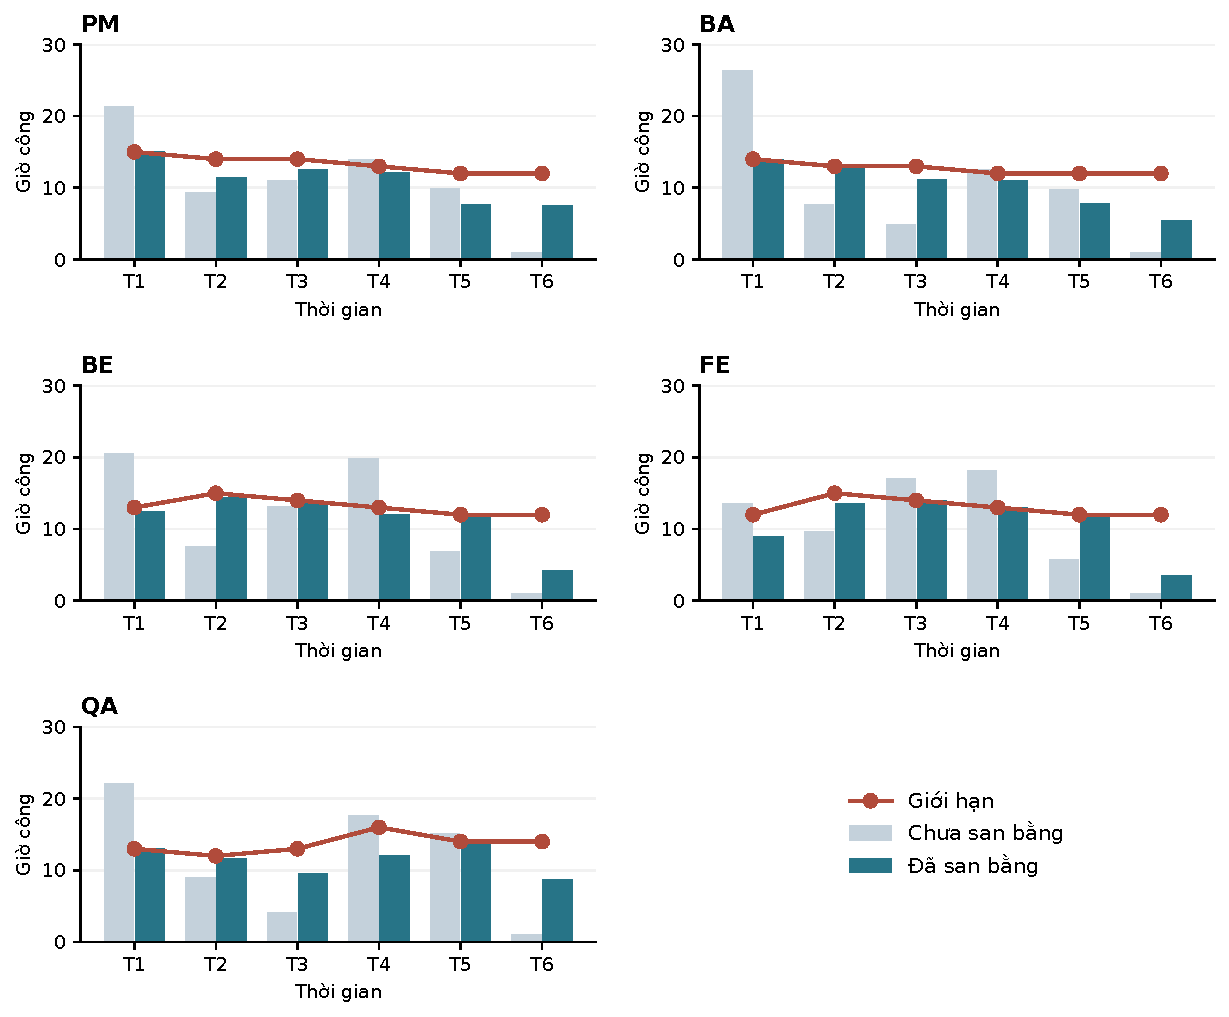
\includegraphics[width=\linewidth]{Images/nguon_luc.pdf}
\caption{Biểu đồ phân bổ Workload nhân sự theo tuần sau Resource Leveling}
\label{fig:resource}
\end{figure}

Kế hoạch phân bổ chính thức ghi nhận dòng công sức theo tuần từ Tuần 1 đến Tuần 6 lần lượt là: 63,5; 64,0; 61,1; 60,2; 53,4 và 29,4 giờ công. Hình \ref{fig:resource} minh họa tính hợp lệ của lịch trình khi toàn bộ cột Workload thực tế đều nằm trong giới hạn Capacity.

\subsubsection{Đánh giá phương án dời tiến độ}

Nhóm đã thử nghiệm kiểm định kịch bản Nén tiến độ (Schedule Compression): "Dồn toàn bộ khối lượng Tuần 6 về Tuần 5" nhằm kết thúc sớm. Kết quả phân tích tại Bảng 47 cho thấy phương án này gây quá tải nghiêm trọng cho tất cả 5 nhân sự.

\begingroup\small
\setlength{\tabcolsep}{5pt}\renewcommand{\arraystretch}{1.15}
\begin{longtable}{@{}lrrrrr@{}}
\caption{Đánh giá Workload khi nén tiến độ Tuần 6 vào Tuần 5 (Đơn vị: Giờ công)}\label{tab:compression}\\
\toprule
\textbf{Nhân sự} & \textbf{Tải T5 gốc} & \textbf{Chuyển từ T6} & \textbf{Total Workload T5} & \textbf{Capacity T5} & \textbf{Over-allocated} \\
\midrule\endfirsthead
\toprule
\textbf{Nhân sự} & \textbf{Tải T5 gốc} & \textbf{Chuyển từ T6} & \textbf{Total Workload T5} & \textbf{Capacity T5} & \textbf{Over-allocated} \\
\midrule\endhead
\bottomrule\endlastfoot
PM & 7,7 & 7,5 & 15,2 & 12,0 & 3,2 \\
BA & 7,8 & 5,5 & 13,3 & 12,0 & 1,3 \\
BE & 12,0 & 4,2 & 16,2 & 12,0 & 4,2 \\
FE & 11,9 & 3,5 & 15,4 & 12,0 & 3,4 \\
QA & 14,0 & 8,7 & 22,7 & 14,0 & 8,7 \\
\end{longtable}\endgroup

Do các tác vụ sau nghiệm thu A12.2 (ngày 30/11) như BL2, A16, A18.2 và A17 đòi hỏi trình tự thực hiện nối tiếp, việc giữ 29,4 giờ công sang Tuần 6 là giải pháp tối ưu, đảm bảo hoàn tất đóng gói hồ sơ và bàn giao sản phẩm chính thức vào ngày 03/12/2026.

\begingroup\small
\setlength{\tabcolsep}{4pt}\renewcommand{\arraystretch}{1.15}
\begin{longtable}{@{}lr@{}}
\caption{Các mốc hoàn thành công việc chính}\label{tab:revised-milestones}\\
\toprule
\textbf{Hạng mục công việc} & \textbf{Ngày hoàn thành kế hoạch} \\
\midrule\endfirsthead
\toprule
\textbf{Hạng mục công việc} & \textbf{Ngày hoàn thành kế hoạch} \\
\midrule\endhead
\midrule\multicolumn{2}{r}{\textit{Còn tiếp}}\\\endfoot
\bottomrule\endlastfoot
Kiểm thử \& sửa lỗi Increment 1 (A06) & 09/11/2026 \\
Kiểm thử \& sửa lỗi Increment 2 (A08) & 19/11/2026 \\
Kiểm thử nghiệm thu Increment 3 (A12.2) & 30/11/2026 \\
Chốt phiên bản \& xác minh User Guide (BL2) & 01/12/2026 \\
Chốt báo cáo quản lý dự án (A18.2) & 02/12/2026 \\
Demo \& Bàn giao sản phẩm chính thức (A17) & 03/12/2026 \\
\end{longtable}\endgroup

\subsubsection{Quản lý Schedule Buffer}

Tổng Capacity khả dụng của nhóm trong 6 tuần là 395,0 giờ công. Chênh lệch 63,4 giờ công giữa Capacity và Baseline ($395{,}0 - 331{,}6$) đóng vai trò là quỹ nguồn lực dự phòng cho các công việc phát sinh.

Khoảng thời gian từ ngày \textbf{04/12 đến 06/12/2026} được thiết lập làm \textbf{Schedule Buffer} (khoảng đệm tiến độ). Khoảng thời gian này dùng để xử lý các yêu cầu chỉnh sửa hoặc hoàn thiện tài liệu sau buổi demo/bàn giao (CP6 ngày 03/12/2026), đảm bảo dự án nộp báo cáo đúng hạn vào ngày 06/12/2026.